%%%%%%%%%%%%%%%%%%%%%%%%%%%%%%%%%%%%%%%%%%%%%%%%%%%%%%%%
\fondo{celeste}
\section{Arquitecturas de CNN}
\fondo{blanco}
%%%%%%%%%%%%%%%%%%%%%%%%%%%%%%%%%%%%%%%%%%%%%%%%%%%%%%%%

%%%%%%%%%%%%%%%%%%%%%%%%%%%%%%%%%%%%%%%%%%%%%%%%%%%%%%%%
\begin{frame}
    \frametitle{LeNet-5}

    \begin{columns}
    
    \column{.4\textwidth}
    \begin{center}
        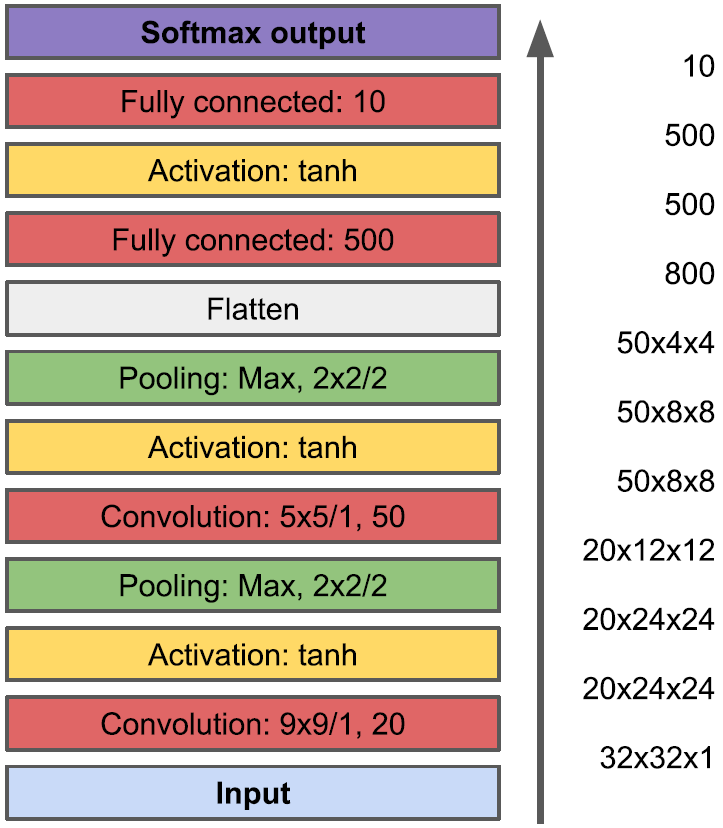
\includegraphics[width=0.9\linewidth]{Figuras/Img12.png}
    \end{center}
    
    \column{.6\textwidth}
    \begin{itemize}
        \item Desarrollada por Bengio et al. en 1998.
        \item Objetivo: reconocimiento de dígitos escritos a mano.
        \item Pequeña y eficiente.
        \item Ideal para aprender y realizar pruebas iniciales.
        \item Puede ejecutarse en una CPU sin necesidad de GPU.
    \end{itemize}

    \end{columns}

\end{frame}
%%%%%%%%%%%%%%%%%%%%%%%%%%%%%%%%%%%%%%%%%%%%%%%%%%%%%%%%


%%%%%%%%%%%%%%%%%%%%%%%%%%%%%%%%%%%%%%%%%%%%%%%%%%%%%%%%
\begin{frame}
\frametitle{AlexNet}
\centering
    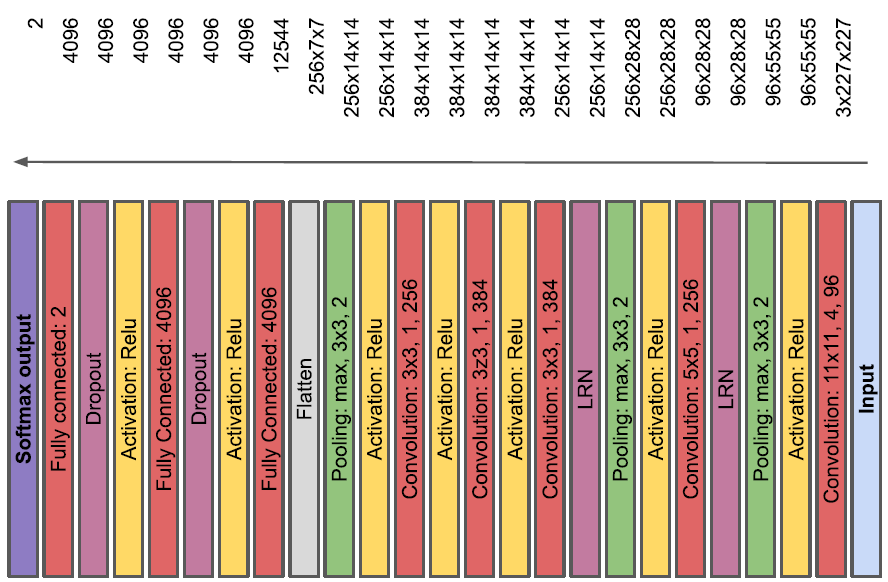
\includegraphics[width=0.65\linewidth]{Figuras/Img13.png}
\end{frame}
%%%%%%%%%%%%%%%%%%%%%%%%%%%%%%%%%%%%%%%%%%%%%%%%%%%%%%%%

%%%%%%%%%%%%%%%%%%%%%%%%%%%%%%%%%%%%%%%%%%%%%%%%%%%%%%%%
\begin{frame}
\frametitle{VGG}
\centering
    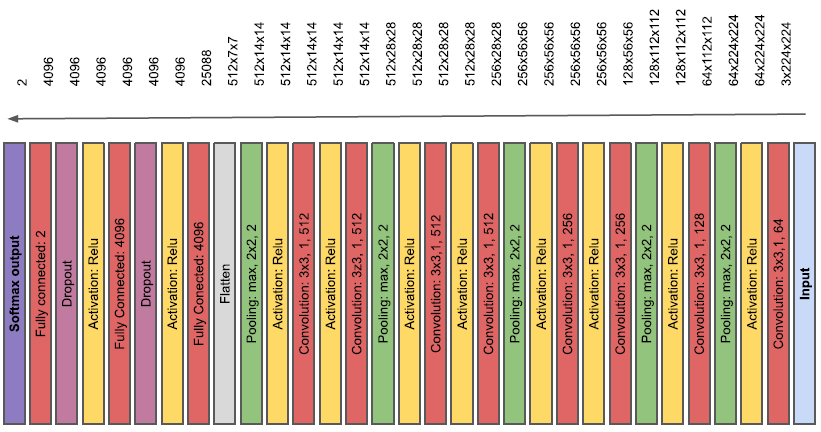
\includegraphics[width=0.8\linewidth]{Figuras/Img14.png}
\end{frame}
%%%%%%%%%%%%%%%%%%%%%%%%%%%%%%%%%%%%%%%%%%%%%%%%%%%%%%%%

%%%%%%%%%%%%%%%%%%%%%%%%%%%%%%%%%%%%%%%%%%%%%%%%%%%%%%%%
\begin{frame}
\frametitle{YOLOv5}
\centering
    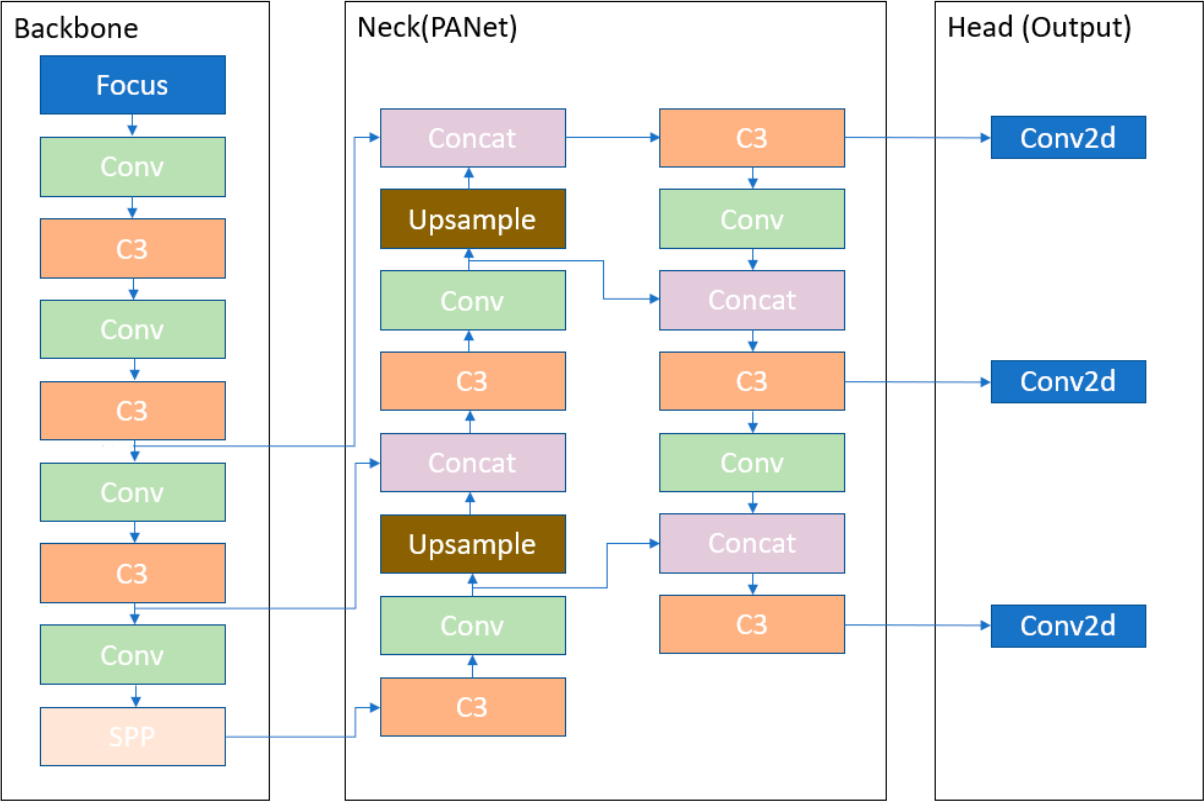
\includegraphics[width=0.65\linewidth]{Figuras/yolov5.png}
\end{frame}
%%%%%%%%%%%%%%%%%%%%%%%%%%%%%%%%%%%%%%%%%%%%%%%%%%%%%%%%


%%%%%%%%%%%%%%%%%%%%%%%%%%%%%%%%%%%%%%%%%%%%%%%%%%%%%%%%
\begin{frame}
    \frametitle{Transferencia del Aprendizaje}

    \begin{itemize}[leftmargin=*]
        \item Permite reutilizar un modelo entrenado en una tarea para aplicarlo en otra tarea similar.
        \item Mejora el rendimiento del modelo y acelera el progreso.
        \item Es popular en **Deep Learning** debido a los altos costos computacionales y de datos necesarios para entrenar modelos desde cero.
        \item La técnica más común es usar un \textbf{modelo pre-entrenado} y adaptarlo:
        \begin{itemize}
            \item Seleccionar el modelo fuente.
            \item Reutilizar todo o parte del modelo.
            \item Ajustar el modelo a la nueva tarea (tunning).
        \end{itemize}
    \end{itemize}

\end{frame}
%%%%%%%%%%%%%%%%%%%%%%%%%%%%%%%%%%%%%%%%%%%%%%%%%%%%%%%%

%%%%%%%%%%%%%%%%%%%%%%%%%%%%%%%%%%%%%%%%%%%%%%%%%%%%%%%%
\begin{frame}
    \frametitle{Técnicas de ajuste (tunning)}

        \begin{itemize}
            \item \textbf{Extracción de características:} usar el modelo como extractor de características.
            \item \textbf{Congelación de capas:} mantener los pesos de algunas capas y reentrenar otras.
        \end{itemize}


\end{frame}
%%%%%%%%%%%%%%%%%%%%%%%%%%%%%%%%%%%%%%%%%%%%%%%%%%%%%%%%
